\documentclass[../presentation.tex]{subfiles} % Parent file
\graphicspath{{\subfix{../images/}}} % Images path

\begin{document}

\section{Datasets}

% Slide 1 ──────────────────────────────────────────────────────────────────────
\begin{frame}

	\frametitle{BraTS 2020 Dataset}

		Segmentation task dataset
		\begin{cbox}
			\begin{itemize}
					\item BraTS stands for Brain Tumor Segmentation
					\item it is composed by $155$ horizontal "slices" of brain MRI images
						for 369 patients (volumes): 
					\[155 \cdot 369 = 57195 \]
				\item we used the $50\%$ ``\itt{most significant}'' slices of the dataset
					\item we used \azure{$90\%$} of data for \azure{training} and
						\green{$10\%$} for \green{testing}
			\end{itemize}
		\end{cbox}

		%TODO: side view of the brain image

\end{frame}

% Slide 2 ──────────────────────────────────────────────────────────────────────
\begin{frame}
    \frametitle{BraTS 2020 Dataset}
    Images have 4 channels:
        \begin{enumerate}
            \item \textbf{T1 weighted (T1)}: \gray{\itt{good for visualizing the
						brain but not the tumor}}
            \item \textbf{T1 weighted with contrast (T1c)}: \gray{\itt{taken
							with the same technique as T1 but with contrast}}
            \item \textbf{T2 weighted (T2)}: \gray{\itt{good for visualizing the
							edema}}
            \item \textbf{Fluid Attenuated Inversion Recovery (FLAIR)}:
							\gray{\itt{improves the visualization of the edema}}
        \end{enumerate}
        \begin{center}
            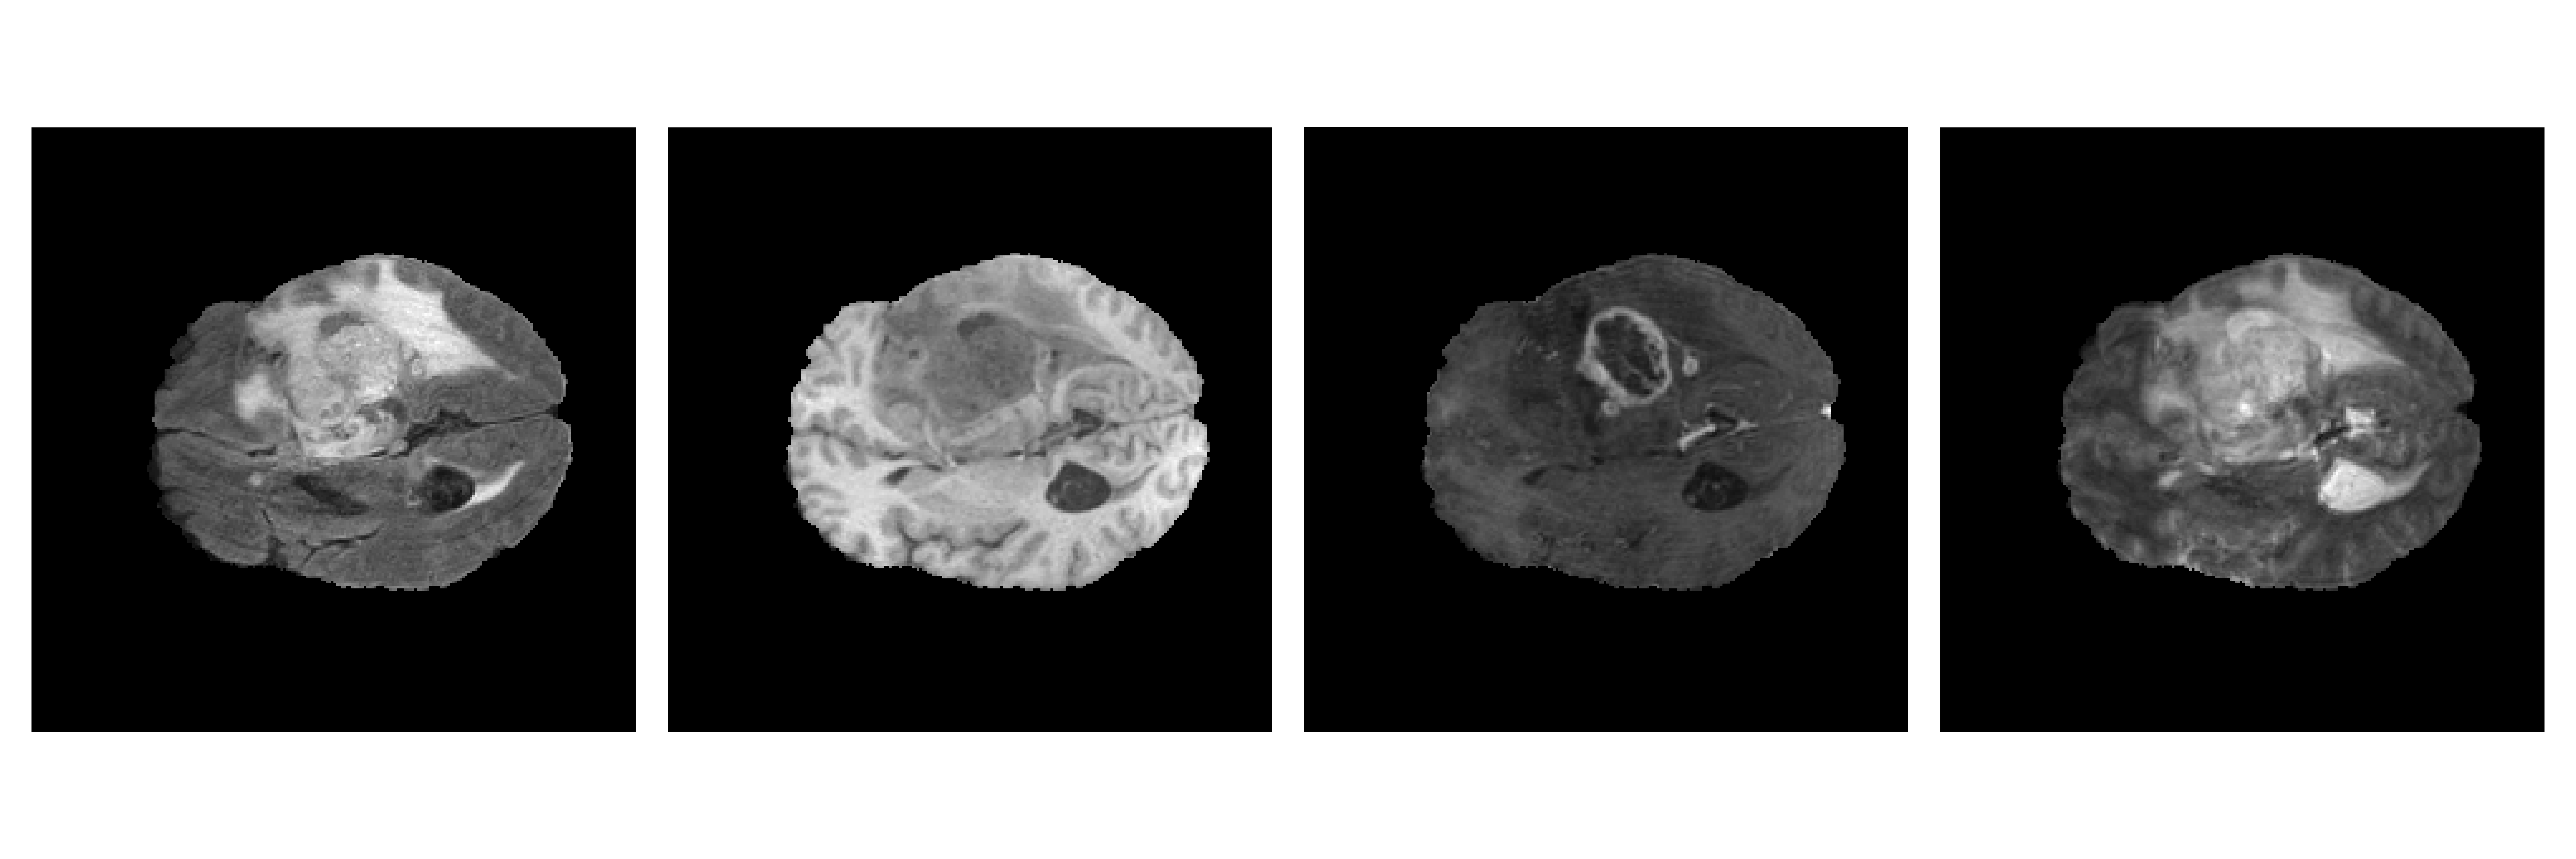
\includegraphics[width=\textwidth]{segmentation_input2.png}
        \end{center}
\end{frame}

% Slide 3 ──────────────────────────────────────────────────────────────────────
\begin{frame}

	\frametitle{BraTS 2020 Dataset}
	Each slice has 3 mask labels \gray{\itt{(some might be empty)}}:
    \begin{enumerate}
			\item \bred{Necrotic and Non-Enhancing Tumor Core (NCR/NET)}
			\item \bgreen{Edema (ED)}
			\item \bblue{Enhancing Tumor (ET)}
    \end{enumerate}
    \begin{center}
        % 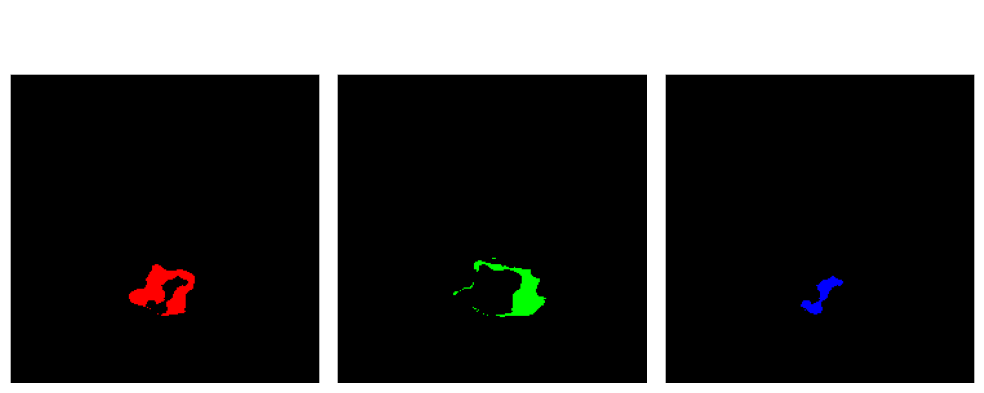
\includegraphics[width=\textwidth]{segmentation-ground-truth.png}
			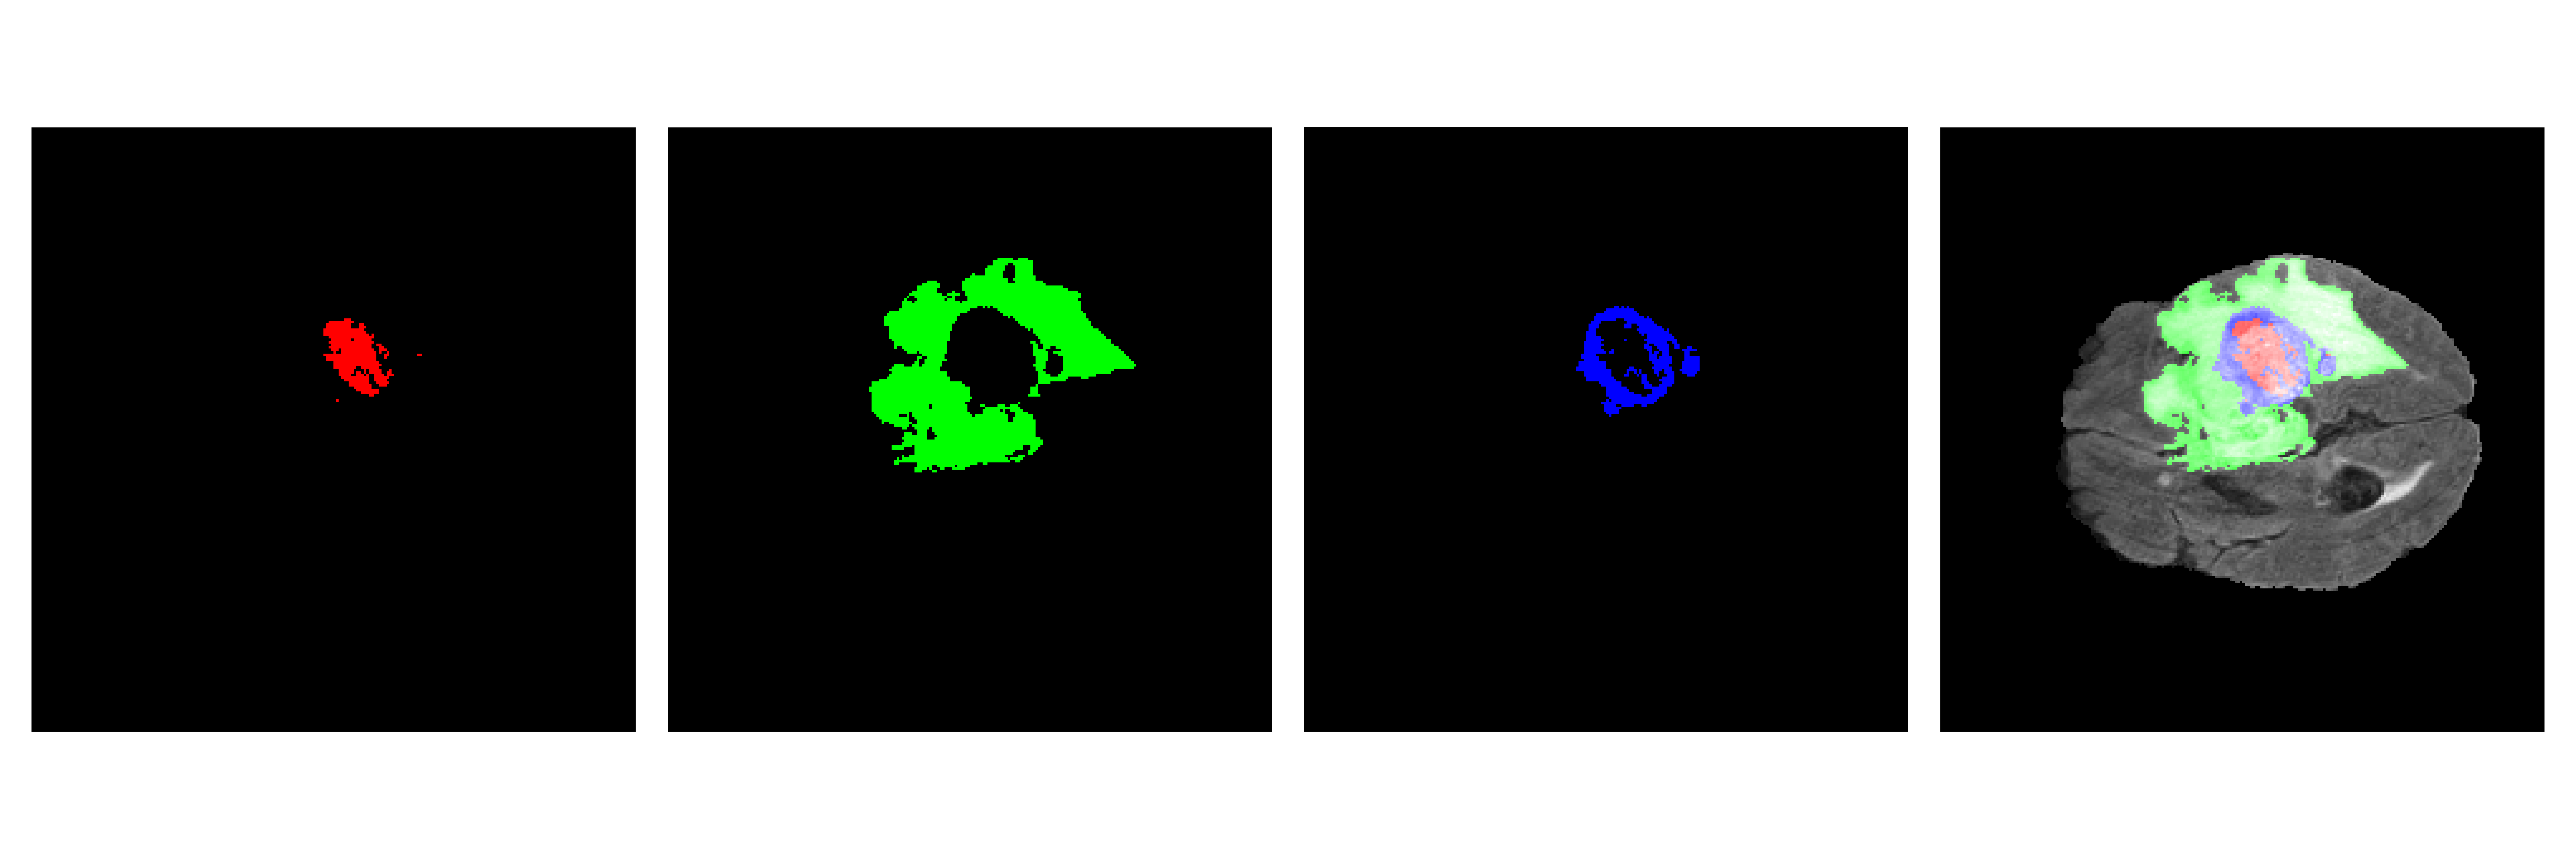
\includegraphics[width=\textwidth]{ground_truth.png}
    \end{center}

\end{frame}

\end{document}
